\documentclass{article}

% content/resources/templates/preamble.tex
\usepackage[margin=0.6in]{geometry}
\author{Milav Dabgar}
\usepackage{amsmath,amssymb,amsthm}
\usepackage{booktabs}
\usepackage{multirow}
\usepackage{xcolor}
\usepackage{tcolorbox}
\tcbuselibrary{breakable,skins}
\usepackage[colorlinks=true,linkcolor=blue]{hyperref}
\usepackage{titlesec}
\usepackage{enumitem}
\usepackage{tikz}
\usepackage{pgfplots}
\usepackage{circuitikz}
\usepackage[version=4]{mhchem}
\usepackage{longtable}
\usepackage{array}
\usepackage{float}
\usepackage{caption}
\usepackage{listings}

\lstset{
  basicstyle=\small\ttfamily,
  breaklines=true,
  breakatwhitespace=false,
  postbreak=\mbox{\textcolor{red}{$\hookrightarrow$}\space},
  float=false,
  numbers=left,
  numberstyle=\tiny\color{gray},
  numbersep=10pt,
  xleftmargin=2em,
  keywordstyle=\color{blue},
  commentstyle=\color{green!60!black},
  stringstyle=\color{purple},
  backgroundcolor=\color{gray!5},
  showstringspaces=false,
  tabsize=2,
  captionpos=b,
  keepspaces=true,
  columns=flexible
}

\pgfplotsset{compat=1.18}
\usetikzlibrary{shapes,arrows,positioning,calc,patterns,decorations.pathmorphing,decorations.markings,arrows.meta}

% Color scheme
\definecolor{headcolor}{RGB}{0,102,204}
\definecolor{keycolor}{RGB}{220,20,60}
\definecolor{solutioncolor}{RGB}{34,139,34}
\definecolor{mnemoniccolor}{RGB}{148,0,211}
\definecolor{codecolor}{RGB}{0,0,100}

% Spacing
\setlength{\parskip}{3pt}
\setlist[itemize]{nosep}
\setlist[enumerate]{nosep}

% Title formatting
\titleformat{\section}{\Large\bfseries\color{headcolor}}{\thesection}{1em}{}
\titleformat{\subsection}{\large\bfseries\color{headcolor}}{\thesubsection}{1em}{}

% Pandoc tightlist compatibility
\providecommand{\tightlist}{%
  \setlength{\itemsep}{0pt}\setlength{\parskip}{0pt}}

% Pandoc longtable compatibility
\newcounter{none}
\def\thenone{}


% content/resources/templates/english-boxes.tex

% Custom environments
\newtcolorbox{solutionbox}{
 breakable,
 enhanced,
 colback=solutioncolor!5!white,
 colframe=solutioncolor!75!black,
 fonttitle=\bfseries,
 title=Solution
}

\newtcolorbox{solutionboxnobreak}{
 colback=solutioncolor!5!white,
 colframe=solutioncolor!75!black,
 fonttitle=\bfseries,
 title=Solution
}

\newtcolorbox{keyformula}{
 breakable,
 enhanced,
 colback=keycolor!5!white,
 colframe=keycolor!75!black,
 fonttitle=\bfseries,
 title=Key Formula
}

\newtcolorbox{mnemonicboxenv}{
 breakable,
 enhanced,
 colback=mnemoniccolor!5!white,
 colframe=mnemoniccolor!75!black,
 fonttitle=\bfseries,
 title=Mnemonic
}

\newcommand{\mnemonicbox}[1]{%
  \begin{mnemonicboxenv}
    #1
  \end{mnemonicboxenv}
}


% Custom commands for GTU solutions
% This file defines semantic commands for consistent formatting

% Question command with automatic formatting
\newcommand{\question}[2]{%
  \section*{Question #1}%
  \textbf{#2}%
}

% OR question variant
\newcommand{\questionor}[2]{%
  \section*{Question #1 OR}%
  \textbf{#2}%
}

% Proper table environment with caption
\newenvironment{answertable}[1]{%
  \begin{table}[htbp]
  \centering
  \caption{#1}
}{%
  \end{table}
}

% Proper figure environment for diagrams
\newenvironment{answerdiagram}[1]{%
  \begin{figure}[htbp]
  \centering
  \caption{#1}
}{%
  \end{figure}
}

% Semantic markup for key terms
\newcommand{\keyword}[1]{\textbf{#1}}
\newcommand{\code}[1]{\texttt{#1}}
\newcommand{\classname}[1]{\texttt{#1}}
\newcommand{\methodname}[1]{\texttt{#1}}

% Proper quotation marks
\newcommand{\mnemonic}[1]{``#1''}


\title{Fundamentals of Electronics (4311102) - Summer 2023 Solution}
\date{July 31, 2023}

\begin{document}
\maketitle

% Question 1
\questionmarks{1(a)}{3}{Define Active and Passive components.}

\begin{solutionbox}
\textbf{Answer}:

\begin{center}
\captionof{table}{Active vs Passive Components}
\begin{tabulary}{\linewidth}{|L|L|}
\hline
\textbf{Active Components} & \textbf{Passive Components} \\ \hline
Require external power source to operate. & Do not need external power source. \\ \hline
Can amplify and process electrical signals. & Cannot amplify or process signals. \\ \hline
\textbf{Examples}: transistors, diodes, ICs. & \textbf{Examples}: resistors, capacitors, inductors. \\ \hline
\end{tabulary}
\end{center}
\end{solutionbox}

\begin{mnemonicbox}
\mnemonic{APE: Active needs Power to Enhance signals}
\end{mnemonicbox}

\questionmarks{1(b)}{4}{State types of capacitors based on materials used.}

\begin{solutionbox}
\textbf{Answer}:

\begin{center}
\captionof{table}{Types of Capacitors Based on Materials}
\begin{tabulary}{\linewidth}{|L|L|L|}
\hline
\textbf{Material Type} & \textbf{Capacitor Type} & \textbf{Typical Applications} \\ \hline
\textbf{Ceramic} & Ceramic disc, multilayer & Bypass, coupling, high frequency \\ \hline
\textbf{Plastic Film} & Polyester, Polypropylene, Teflon & Timing, filtering, precision \\ \hline
\textbf{Electrolytic} & Aluminum, Tantalum & Power supply, DC blocking, high capacitance \\ \hline
\textbf{Paper} & Paper dielectric & Old equipment, not common now \\ \hline
\textbf{Mica} & Silvered mica & High precision RF circuits \\ \hline
\textbf{Glass} & Glass dielectric & High voltage applications \\ \hline
\end{tabulary}
\end{center}
\end{solutionbox}

\begin{mnemonicbox}
\mnemonic{CEPPMG: Ceramic Electrolytic Paper Plastic Mica Glass}
\end{mnemonicbox}

\questionmarks{1(c)}{7}{Explain resistor color coding technique with example.}

\begin{solutionbox}
\textbf{Answer}:

The resistor color code uses colored bands to indicate resistance value, tolerance, and reliability.

\begin{center}
\captionof{table}{Standard Resistor Color Code}
\begin{tabulary}{\linewidth}{|L|C|L|L|}
\hline
\textbf{Color} & \textbf{Digit} & \textbf{Multiplier} & \textbf{Tolerance} \\ \hline
Black & 0 & $\times 10^0$ (1) & - \\ \hline
Brown & 1 & $\times 10^1$ (10) & $\pm 1\%$ \\ \hline
Red & 2 & $\times 10^2$ (100) & $\pm 2\%$ \\ \hline
Orange & 3 & $\times 10^3$ (1k) & - \\ \hline
Yellow & 4 & $\times 10^4$ (10k) & - \\ \hline
Green & 5 & $\times 10^5$ (100k) & $\pm 0.5\%$ \\ \hline
Blue & 6 & $\times 10^6$ (1M) & $\pm 0.25\%$ \\ \hline
Violet & 7 & $\times 10^7$ (10M) & $\pm 0.1\%$ \\ \hline
Grey & 8 & $\times 10^8$ & $\pm 0.05\%$ \\ \hline
White & 9 & $\times 10^9$ & - \\ \hline
Gold & - & $\times 0.1$ & $\pm 5\%$ \\ \hline
Silver & - & $\times 0.01$ & $\pm 10\%$ \\ \hline
\end{tabulary}
\end{center}

\begin{answerdiagram}{Resistor Color Bands}
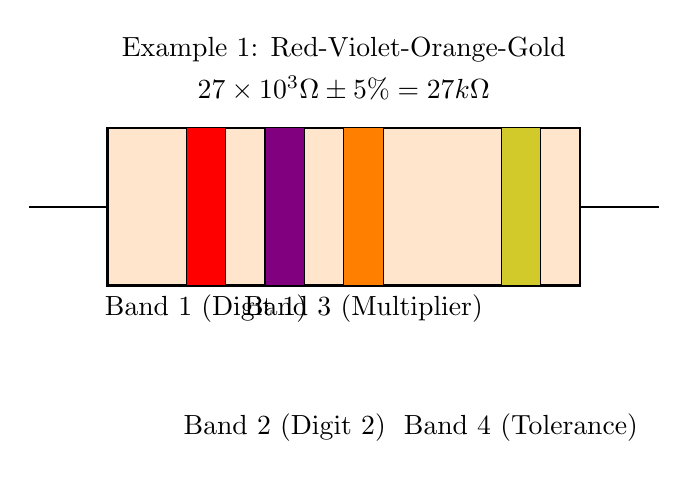
\begin{tikzpicture}
    \draw[thick, fill=orange!20] (0,0) rectangle (6,2);
    \draw[thick] (-1,1) -- (0,1);
    \draw[thick] (6,1) -- (7,1);
    
    % Bands
    \draw[fill=red] (1,0) rectangle (1.5,2) node[midway, below=1cm] {Band 1 (Digit 1)};
    \draw[fill=violet] (2,0) rectangle (2.5,2) node[midway, below=2.5cm] {Band 2 (Digit 2)};
    \draw[fill=orange] (3,0) rectangle (3.5,2) node[midway, below=1cm] {Band 3 (Multiplier)};
    \draw[fill=yellow!80!black] (5,0) rectangle (5.5,2) node[midway, below=2.5cm] {Band 4 (Tolerance)};
    
    % Example
    \node at (3, 3) {Example 1: Red-Violet-Orange-Gold};
    \node at (3, 2.5) {$27 \times 10^3 \Omega \pm 5\% = 27k\Omega$};
\end{tikzpicture}
\end{answerdiagram}

\textbf{Example 1:} Red-Violet-Orange-Gold
\begin{itemize}
    \item 1st (Red) = 2, 2nd (Violet) = 7, 3rd (Orange) = $\times 1k$, 4th (Gold) = $\pm 5\%$
    \item Value: $27k\Omega \pm 5\%$
\end{itemize}

\textbf{Example 2:} Brown-Black-Yellow-Silver
\begin{itemize}
    \item 1st (Brown) = 1, 2nd (Black) = 0, 3rd (Yellow) = $\times 10k$, 4th (Silver) = $\pm 10\%$
    \item Value: $100k\Omega \pm 10\%$
\end{itemize}
\end{solutionbox}

\begin{mnemonicbox}
\mnemonic{BBROY: BBROY Great Britain Very Good Wife (Black Brown Red Orange Yellow Green Blue Violet Gray White)}
\end{mnemonicbox}

% Question 1 OR
\questionmarks{1(c) OR}{7}{Explain construction, working Characteristic and application of LDR.}

\begin{solutionbox}
\textbf{Answer}:

\textbf{Light Dependent Resistor (LDR)}

\begin{center}
\captionof{table}{LDR Details}
\begin{tabulary}{\linewidth}{|L|L|}
\hline
\textbf{Aspect} & \textbf{Description} \\ \hline
\textbf{Construction} & Semiconductor material (cadmium sulfide) deposited in zigzag pattern on ceramic substrate. Packaged in transparent case with two terminals. \\ \hline
\textbf{Working Principle} & Photoconductivity: When light falls on material, photons release electron-hole pairs, increasing conductivity and decreasing resistance. \\ \hline
\textbf{Characteristics} & High resistance in dark (M$\Omega$). Low resistance in light (100-5000$\Omega$). Inverse non-linear relationship. Slow response time. \\ \hline
\textbf{Applications} & Automatic street lights, camera light meters, burglar alarms, display brightness control. \\ \hline
\end{tabulary}
\end{center}

\begin{answerdiagram}{LDR Characteristics and Symbol}
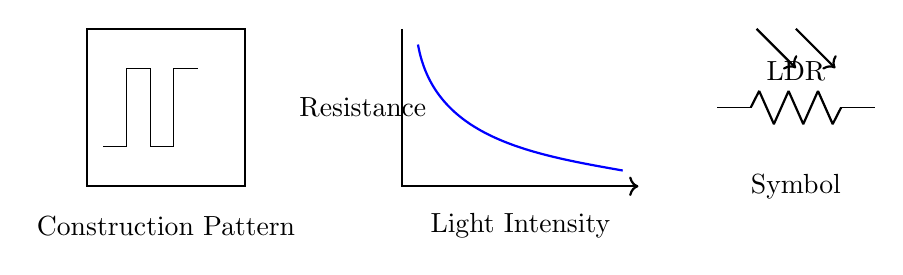
\begin{tikzpicture}
    \begin{scope}[xshift=0cm]
        \draw[thick] (0,0) rectangle (2,2);
        \draw (0.2, 0.5) -- (0.5, 0.5) -- (0.5, 1.5) -- (0.8, 1.5) -- (0.8, 0.5) -- (1.1, 0.5) -- (1.1, 1.5) -- (1.4, 1.5);
        \node at (1, -0.5) {Construction Pattern};
    \end{scope}

    \begin{scope}[xshift=4cm]
        \draw[thick, ->] (0,2) -- (0,0) -- (3,0);
        \node at (1.5, -0.5) {Light Intensity};
        \node at (-0.5, 1) {Resistance};
        \draw[blue, thick] (0.2, 1.8) to[out=-80, in=170] (2.8, 0.2);
    \end{scope}
    
    \begin{scope}[xshift=8cm, yshift=1cm]
         \draw (0,0) to[R, l=LDR] (2,0);
         \draw[->, thick] (0.5, 1) -- (1, 0.5);
         \draw[->, thick] (1, 1) -- (1.5, 0.5);
         \node at (1, -1) {Symbol};
    \end{scope}
\end{tikzpicture}
\end{answerdiagram}
\end{solutionbox}

\begin{mnemonicbox}
\mnemonic{MOLD: More light On, Less resistance Down}
\end{mnemonicbox}

% Question 2
\questionmarks{2(a)}{3}{Classify Resistors based on materials.}

\begin{solutionbox}
\textbf{Answer}:

\begin{center}
\captionof{table}{Resistor Classification}
\begin{tabulary}{\linewidth}{|L|L|L|}
\hline
\textbf{Material Type} & \textbf{Characteristics} & \textbf{Examples} \\ \hline
\textbf{Carbon Composition} & Low cost, noisy, poor tolerance. & General purpose. \\ \hline
\textbf{Carbon Film} & Better stability than composition. & Audio, general circuits. \\ \hline
\textbf{Metal Film} & Excellent stability, low noise. & Precision circuits. \\ \hline
\textbf{Metal Oxide} & Heat resistant, high stability. & Power supplies. \\ \hline
\textbf{Wire Wound} & High power, inductive. & Heating elements. \\ \hline
\textbf{Thick/Thin Film} & Small size (SMD). & Surface mount. \\ \hline
\end{tabulary}
\end{center}
\end{solutionbox}

\begin{mnemonicbox}
\mnemonic{CMMWTF: Carbon Makes Much Wire To Form resistors}
\end{mnemonicbox}

\questionmarks{2(b)}{4}{Calculate value of resistor for a given color code. – (i) Brown, Black, Yellow, Golden (ii) Yellow, Violet, Red, Silver}

\begin{solutionbox}
\textbf{Answer}:

\textbf{Part (i): Brown, Black, Yellow, Golden}
\begin{itemize}
    \item Brown (1), Black (0), Yellow ($\times 10^4$), Golden ($\pm 5\%$)
    \item $10 \times 10,000 = 100,000\Omega = 100k\Omega \pm 5\%$
\end{itemize}

\textbf{Part (ii): Yellow, Violet, Red, Silver}
\begin{itemize}
    \item Yellow (4), Violet (7), Red ($\times 10^2$), Silver ($\pm 10\%$)
    \item $47 \times 100 = 4,700\Omega = 4.7k\Omega \pm 10\%$
\end{itemize}
\end{solutionbox}

\questionmarks{2(c)}{7}{Illustrate construction and operation of Electrolytic capacitors.}

\begin{solutionbox}
\textbf{Answer}:

\begin{center}
\captionof{table}{Electrolytic Capacitor}
\begin{tabulary}{\linewidth}{|L|L|}
\hline
\textbf{Component} & \textbf{Description} \\ \hline
\textbf{Anode} & Aluminum foil with oxide layer (dielectric). \\ \hline
\textbf{Cathode} & Electrolyte (liquid/paste) and metal foil. \\ \hline
\textbf{Separator} & Paper soaked in electrolyte. \\ \hline
\textbf{Operation} & Oxide layer gives high capacitance ($C \propto A/d$) due to extreme thinness. Polarized (must connect correct +/-). \\ \hline
\end{tabulary}
\end{center}

\begin{answerdiagram}{Electrolytic Capacitor Construction}
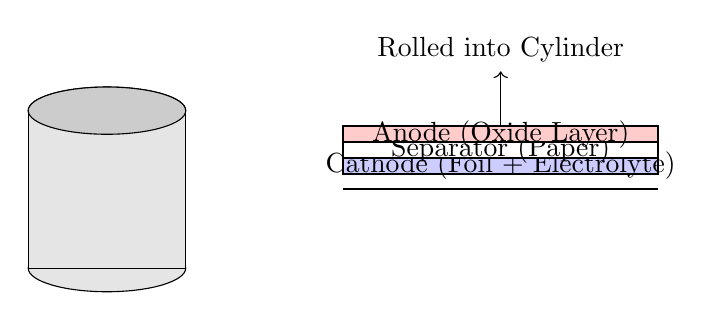
\begin{tikzpicture}
    % Capacitor Can (Cylinder)
    \draw[fill=gray!20] (0,2) ellipse (1 and 0.3);
    \draw[fill=gray!20] (0,0) ellipse (1 and 0.3);
    \draw[fill=gray!20] (-1,0) rectangle (1,2);
    \draw[fill=gray!40] (0,2) ellipse (1 and 0.3); % Top cap
    \draw (-1,0) -- (-1,2);
    \draw (1,0) -- (1,2);
    
    % Internal layers roll
    \begin{scope}[xshift=3cm, yshift=1cm]
        \draw[thick] (0,0) -- (4,0);
        \draw[thick, fill=blue!20] (0,0.2) rectangle (4,0.4) node[midway] {Cathode (Foil + Electrolyte)};
        \draw[thick, fill=white] (0,0.4) rectangle (4,0.6) node[midway] {Separator (Paper)};
        \draw[thick, fill=red!20] (0,0.6) rectangle (4,0.8) node[midway] {Anode (Oxide Layer)};
        \draw[->] (2,0.8) -- (2,1.5) node[above] {Rolled into Cylinder};
    \end{scope}
\end{tikzpicture}
\end{answerdiagram}
\end{solutionbox}

\begin{mnemonicbox}
\mnemonic{PAVE: Polarized Aluminum with Very high capacitance and Electrolyte}
\end{mnemonicbox}

% Question 2 OR
\questionmarks{2(a) OR}{3}{State the importance of filter circuit in rectifier.}

\begin{solutionbox}
\textbf{Answer}:

\begin{itemize}
    \item \keyword{Smoothing}: Converts pulsating DC from rectifier into steady DC.
    \item \keyword{Ripple Reduction}: Removes unwanted AC components (ripples).
    \item \keyword{Voltage Stabilization}: Maintains average output voltage.
    \item \keyword{device Protection}: Prevents damage to sensitive electronic components.
\end{itemize}
\end{solutionbox}

\begin{mnemonicbox}
\mnemonic{SVRL: Smoothens Voltage by Reducing ripples for Load}
\end{mnemonicbox}

\questionmarks{2(b) OR}{4}{Differentiate between P type semiconductor and N type semiconductor.}

\begin{solutionbox}
\textbf{Answer}:

\begin{center}
\captionof{table}{P-type vs N-type}
\begin{tabulary}{\linewidth}{|L|L|L|}
\hline
\textbf{Feature} & \textbf{P-type} & \textbf{N-type} \\ \hline
\textbf{Dopant} & Trivalent (B, Al, Ga) & Pentavalent (P, As, Sb) \\ \hline
\textbf{Majority Carriers} & Holes (+) & Electrons (-) \\ \hline
\textbf{Minority Carriers} & Electrons (-) & Holes (+) \\ \hline
\textbf{Energy Level} & Acceptor level near Valence band & Donor level near Conduction band \\ \hline
\end{tabulary}
\end{center}
\end{solutionbox}

\begin{mnemonicbox}
\mnemonic{HELP-NED: Holes Exist Large in P, Negative Electrons Dominate N}
\end{mnemonicbox}

\questionmarks{2(c) OR}{7}{Illustrate working of Bridge Rectifier with waveforms.}

\begin{solutionbox}
\textbf{Answer}:

\textbf{Operation}:
\begin{itemize}
    \item \keyword{Positive Half}: D1, D3 conduct. Current flows through load.
    \item \keyword{Negative Half}: D2, D4 conduct. Current flows through load in same direction.
    \item \keyword{Result}: Full wave rectification without center-tap transformer.
\end{itemize}

\begin{answerdiagram}{Bridge Rectifier Circuit and Waveforms}
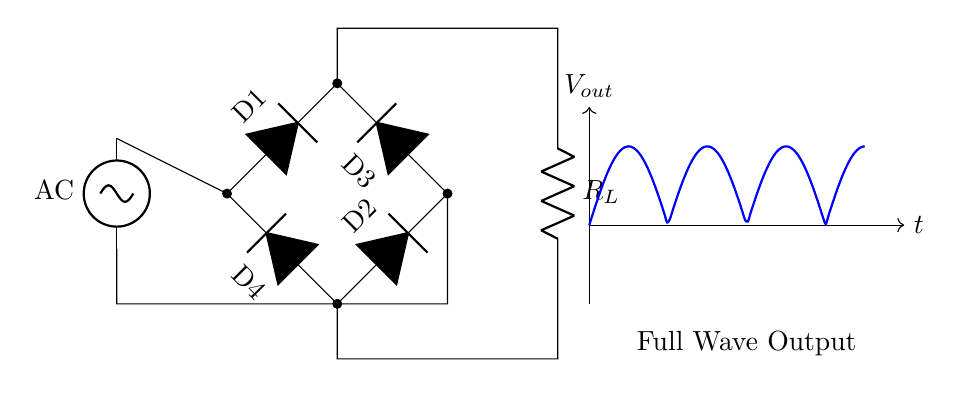
\begin{tikzpicture}
    % Circuit
    \begin{scope}[scale=0.7]
        \coordinate (L) at (2, 2);
        \coordinate (R) at (6, 2);
        \coordinate (T) at (4, 4);
        \coordinate (B) at (4, 0);
        
        % Diodes (D1: L->T, D3: R->T, D4: B->L, D2: B->R)
        \draw (L) to[D*, l=D1] (T);
        \draw (R) to[D*, l=D3] (T);
        \draw (B) to[D*, l=D4] (L);
        \draw (B) to[D*, l=D2] (R);
        
        % AC Source
        \draw (0,1) to[sV, l=AC] (0,3);
        \draw (0,3) -- (L);
        \draw (0,1) -- (0,0) -- (6,0) -- (R);
        
        % Load
        \draw (T) -- (4,5) -- (8,5) to[R, l=$R_L$] (8,-1) -- (4,-1) -- (B);
        
        % Nodes
        \draw (L) node[circ]{}; \draw (R) node[circ]{};
        \draw (T) node[circ]{}; \draw (B) node[circ]{};
    \end{scope}

    % Waveforms
    \begin{scope}[xshift=6cm, yshift=0cm]
        \draw[->] (0,1) -- (4,1) node[right] {$t$};
        \draw[->] (0,0) -- (0,2.5) node[above] {$V_{out}$};
        \draw[blue, thick, smooth, samples=100, domain=0:3.5] plot (\x, {1 + abs(sin(\x*180))});
        \node at (2, -0.5) {Full Wave Output};
    \end{scope}
\end{tikzpicture}
\end{answerdiagram}
\end{solutionbox}

\begin{mnemonicbox}
\mnemonic{FBRO: Four diodes, Both cycles, Rectified Output}
\end{mnemonicbox}

% Question 3
\questionmarks{3(a)}{3}{Define (1) PIV (2) Ripple Factor.}

\begin{solutionbox}
\textbf{Answer}:

\begin{center}
\captionof{table}{PIV and Ripple Factor}
\begin{tabulary}{\linewidth}{|L|L|}
\hline
\textbf{Term} & \textbf{Definition} \\ \hline
\textbf{PIV (Peak Inverse Voltage)} & Maximum voltage a diode can withstand in reverse bias. Must be higher than circuit's max reverse voltage to prevent breakdown. \\ \hline
\textbf{Ripple Factor (r)} & Ratio of RMS value of AC component to DC component in output. Lower r means better filtering. \\ \hline
\end{tabulary}
\end{center}

\textbf{Formula}: $r = \frac{V_{rms(ac)}}{V_{dc}}$
\end{solutionbox}

\begin{mnemonicbox}
\mnemonic{PIR: Peak Inverse voltage Restricts, Ripple indicates Rectification quality}
\end{mnemonicbox}

\questionmarks{3(b)}{4}{Illustrate VI characteristics of PN junction diode.}

\begin{solutionbox}
\textbf{Answer}:

\begin{center}
\captionof{table}{PN Junction Characteristics}
\begin{tabulary}{\linewidth}{|L|L|}
\hline
\textbf{Region} & \textbf{Behavior} \\ \hline
\textbf{Forward Bias} & Conducts current easily after threshold (0.7V Si, 0.3V Ge). Exponential current rise. \\ \hline
\textbf{Reverse Bias} & Blocks current. Very small leakage ($\mu$A). Breakdown at high reverse voltage. \\ \hline
\end{tabulary}
\end{center}

\begin{answerdiagram}{VI Characteristics of PN Diode}
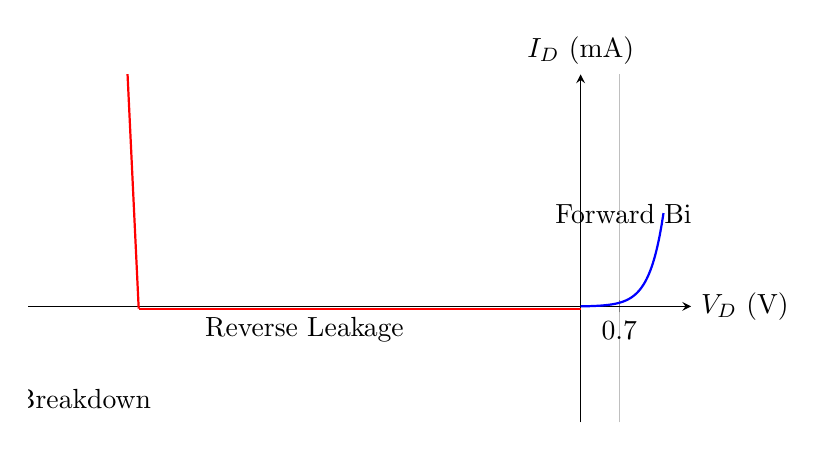
\begin{tikzpicture}
    \begin{axis}[
        axis lines=middle,
        xlabel={$V_D$ (V)}, ylabel={$I_D$ (mA)},
        xmin=-10, xmax=2,
        ymin=-5, ymax=10,
        xtick={0.7}, xticklabels={0.7},
        ytick=\empty,
        width=10cm, height=6cm,
        grid=major,
        every axis x label/.style={at={(current axis.right of origin)},anchor=west},
        every axis y label/.style={at={(current axis.above origin)},anchor=south},
    ]
        % Forward
        \addplot[blue, thick, domain=0:1.5, samples=100] {0.01*(exp(4*x)-1)};
        \node at (axis cs: 1, 4) {Forward Bias};

        % Reverse
        \addplot[red, thick, domain=-8:0] {-0.1}; % Leakage
        \addplot[red, thick, domain=-10:-8] {-50*(x+8)-0.1}; % Breakdown
        \node at (axis cs: -5, -1) {Reverse Leakage};
        \node at (axis cs: -9, -4) {Breakdown};
    \end{axis}
\end{tikzpicture}
\end{answerdiagram}
\end{solutionbox}

\begin{mnemonicbox}
\mnemonic{FBRL: Forward Bias Resists Little, reverse blocks lots}
\end{mnemonicbox}

\questionmarks{3(c)}{7}{Explain the working of capacitor input and choke input filter with waveforms.}

\begin{solutionbox}
\textbf{Answer}:

\textbf{1. Capacitor Input Filter}
\begin{itemize}
    \item Capacitor connected in parallel with load.
    \item Charges to peak, discharges slowly during dips.
    \item High DC voltage, but poor regulation.
\end{itemize}

\textbf{2. Choke Input Filter}
\begin{itemize}
    \item Inductor (choke) in series, capacitor in parallel.
    \item Inductor opposes current change, smoothing current.
    \item Better regulation, lower DC voltage.
\end{itemize}

\begin{answerdiagram}{Filter Circuits and Waveforms}
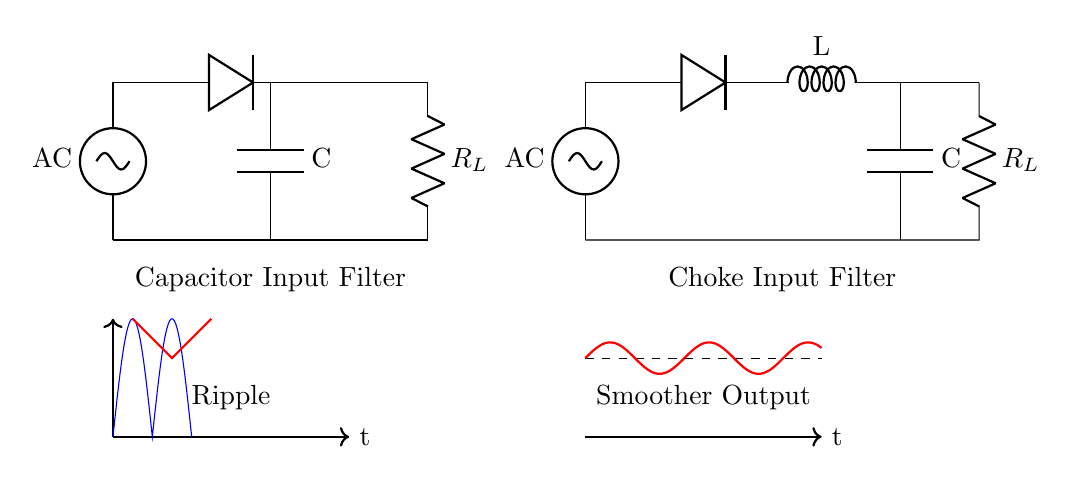
\begin{tikzpicture}
    % Capacitor Filter
    \begin{scope}[xshift=0cm]
        \draw (0,0) to[sV, l=AC] (0,2) -- (1,2) to[D] (2,2) -- (4,2);
        \draw (2,2) to[C, l=C] (2,0);
        \draw (4,2) to[R, l=$R_L$] (4,0) -- (0,0);
        \node at (2, -0.5) {Capacitor Input Filter};
        
        % Waveform
        \draw[thick, ->] (0,-2.5) -- (3,-2.5) node[right] {t};
        \draw[thick, ->] (0,-2.5) -- (0,-1);
        \draw[blue] (0,-2.5) sin (0.25,-1) cos (0.5,-2.5) sin (0.75,-1) cos (1,-2.5);
        \draw[red, thick] (0.25,-1) -- (0.75,-1.5) -- (1.25,-1);
        \node at (1.5, -2) {Ripple};
    \end{scope}

    % Choke Filter
    \begin{scope}[xshift=6cm]
        \draw (0,0) to[sV, l=AC] (0,2) -- (1,2) to[D] (2,2) to[L, l=L] (4,2) -- (5,2);
        \draw (4,2) to[C, l=C] (4,0);
        \draw (5,2) to[R, l=$R_L$] (5,0) -- (0,0);
        \node at (2.5, -0.5) {Choke Input Filter};
        
        % Waveform
        \draw[thick, ->] (0,-2.5) -- (3,-2.5) node[right] {t};
        \draw[dashed] (0,-1.5) -- (3,-1.5);
        \draw[red, thick, smooth] plot[domain=0:3, samples=50] (\x, {-1.5 + 0.2*sin(deg(\x*5))});
        \node at (1.5, -2) {Smoother Output};
    \end{scope}
\end{tikzpicture}
\end{answerdiagram}
\end{solutionbox}

\begin{mnemonicbox}
\mnemonic{VOICE: Voltage Output Is Constant with Either filter, but choke gives better regulation}
\end{mnemonicbox}

% Question 3 OR
\questionmarks{3(a) OR}{3}{State the function and importance of Zener diode.}

\begin{solutionbox}
\textbf{Answer}:

\begin{center}
\captionof{table}{Zener Diode Functions}
\begin{tabulary}{\linewidth}{|L|L|}
\hline
\textbf{Function} & \textbf{Description} \\ \hline
\textbf{Voltage Regulation} & Maintains constant output voltage. \\ \hline
\textbf{Voltage Reference} & Provides precise reference voltage. \\ \hline
\textbf{Protection} & Prevents voltage spikes from damaging circuits. \\ \hline
\textbf{Usage} & Operates in breakdown region. \\ \hline
\end{tabulary}
\end{center}
\end{solutionbox}

\begin{mnemonicbox}
\mnemonic{VPRVW: Voltage Protection, Regulation, and Voltage Waveform control}
\end{mnemonicbox}

\questionmarks{3(b) OR}{4}{Describe Light emitting diode (LED) with its characteristic.}

\begin{solutionbox}
\textbf{Answer}:

\begin{center}
\captionof{table}{LED Characteristics}
\begin{tabulary}{\linewidth}{|L|L|}
\hline
\textbf{Aspect} & \textbf{Description} \\ \hline
\textbf{Principle} & Electroluminescence. Recombination of holes and electrons releases photons. \\ \hline
\textbf{Material} & Direct bandgap semiconductors (GaAs, GaP). \\ \hline
\textbf{Forward Voltage} & Red: ~2V, Blue/White: ~3V. \\ \hline
\textbf{Operation} & Works only in Forward Bias. Damaged by reverse bias ($>5V$). \\ \hline
\end{tabulary}
\end{center}

\begin{answerdiagram}{LED Working}
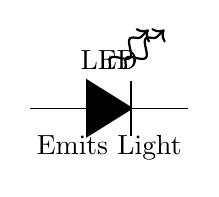
\begin{tikzpicture}
    \draw (0,0) to[D*, l=LED, fill=red] (2,0);
    \draw[->, thick, decorate, decoration={snake}] (1,0.5) -- (1.5, 1);
    \draw[->, thick, decorate, decoration={snake}] (1.2,0.5) -- (1.7, 1);
    \node at (1, -0.5) {Emits Light};
\end{tikzpicture}
\end{answerdiagram}
\end{solutionbox}

\begin{mnemonicbox}
\mnemonic{CRAVE: Current Regulated And Voltage Emits light}
\end{mnemonicbox}

\questionmarks{3(c) OR}{7}{Illustrate the working of capacitor input and choke input filter.}

\begin{solutionbox}
\textbf{Answer}:

\textit{(Refer to Question 3(c) for detailed waveforms and diagrams. This section provides component breakdown.)}

\begin{center}
\captionof{table}{Capacitor vs Choke Filter}
\begin{tabulary}{\linewidth}{|L|L|L|}
\hline
\textbf{Parameter} & \textbf{Capacitor Input} & \textbf{Choke Input} \\ \hline
\textbf{Components} & Capacitor in parallel. & Choke (series) + Cap (parallel). \\ \hline
\textbf{Output V} & Higher ($\approx V_m$). & Lower ($\approx 0.9 V_m$). \\ \hline
\textbf{Regulation} & Poor (V drops with load). & Good (L opposes change). \\ \hline
\textbf{Diode Current} & High peak surges. & Continuous, lower peak. \\ \hline
\textbf{Cost/Size} & Low cost, small. & Heavy, bulky, expensive. \\ \hline
\end{tabulary}
\end{center}
\end{solutionbox}

\begin{mnemonicbox}
\mnemonic{CHEER: Capacitor Holds Energy, inductor Ensures Regulated current}
\end{mnemonicbox}

% Question 4
\questionmarks{4(a)}{3}{Discuss characteristics of PN junction diode.}

\begin{solutionbox}
\textbf{Answer}:

\begin{itemize}
    \item \keyword{Forward Bias}: Low resistance, current flows after knee voltage.
    \item \keyword{Reverse Bias}: High resistance, only leakage current.
    \item \keyword{Breakdown}: Rapid current increase at Zener/Avalanche voltage.
    \item \keyword{Temp Effect}: $V_f$ drops with heat, $I_r$ doubles every $10^\circ$C.
\end{itemize}
\end{solutionbox}

\begin{mnemonicbox}
\mnemonic{FRBCT: Forward conducts, Reverse blocks, Breakdown destroys}
\end{mnemonicbox}

\questionmarks{4(b)}{4}{Compare between P-N junction diode and Zener diode.}

\begin{solutionbox}
\textbf{Answer}:

\begin{center}
\captionof{table}{General Diode vs Zener Diode}
\begin{tabulary}{\linewidth}{|L|L|L|}
\hline
\textbf{Feature} & \textbf{PN Diode} & \textbf{Zener Diode} \\ \hline
\textbf{Symbol} & Standard arrow & Arrow with 'Z' ends \\ \hline
\textbf{Doping} & Moderate & Heavy \\ \hline
\textbf{Breakdown} & Destructive & Non-destructive (Operating region) \\ \hline
\textbf{Main Use} & Rectification & Voltage Regulation \\ \hline
\end{tabulary}
\end{center}
\end{solutionbox}

\begin{mnemonicbox}
\mnemonic{FORBAR: Forward Operation is Regular, Breakdown Application is Real difference}
\end{mnemonicbox}

\questionmarks{4(c)}{7}{Illustrate the function of Zener diode as a voltage regulator.}

\begin{solutionbox}
\textbf{Answer}:

\textbf{Circuit Operation}:
\begin{itemize}
    \item Zener diode connected in \keyword{Reverse Bias}.
    \item When $V_{in} > V_z$, Zener conducts and holds $V_{out} = V_z$.
    \item Series resistor $R_s$ drops the excess voltage ($V_{in} - V_z$).
    \item Changes in load current or input voltage are compensated by changing Zener current, keeping $V_{out}$ steady.
\end{itemize}

\begin{answerdiagram}{Zener Regulator}
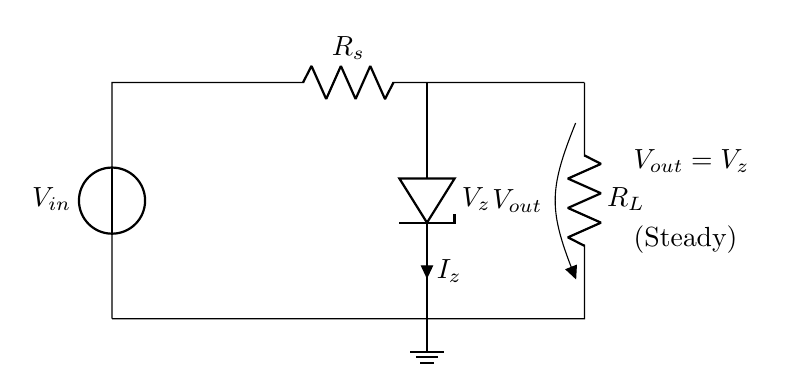
\begin{tikzpicture}
    \draw (0,0) to[V, l=$V_{in}$] (0,3) -- (2,3) to[R, l=$R_s$] (4,3) -- (6,3);
    \draw (4,3) to[zD, l=$V_z$, i=$I_z$] (4,0);
    \draw (6,3) to[R, l=$R_L$, v=$V_{out}$] (6,0) -- (0,0);
    \draw (4,0) node[ground]{};
    
    % Annotations
    \node[right] at (6.5, 2) {$V_{out} = V_z$};
    \node[right] at (6.5, 1) {(Steady)};
\end{tikzpicture}
\end{answerdiagram}
\end{solutionbox}

\begin{mnemonicbox}
\mnemonic{VISOR: Voltage In Stays Out Regulated}
\end{mnemonicbox}

% Question 4 OR
\questionmarks{4(a) OR}{3}{Discuss transistor in brief.}

\begin{solutionbox}
\textbf{Answer}:

\begin{itemize}
    \item \keyword{Definition}: 3-terminal semiconductor device (Emitter, Base, Collector).
    \item \keyword{Types}: BJT (NPN, PNP), FET (JFET, MOSFET).
    \item \keyword{Function}: Amplifies weak signals, acts as a switch.
    \item \keyword{Control}: Current controlled (BJT) or Voltage controlled (FET).
\end{itemize}
\end{solutionbox}

\begin{mnemonicbox}
\mnemonic{TAWAI: Transistors Amplify, Work As switches, and are Integral}
\end{mnemonicbox}

\questionmarks{4(b) OR}{4}{Derive relation between $\alpha$ and $\beta$ for transistor amplifier.}

\begin{solutionbox}
\textbf{Answer}:

\textbf{Definitions}:
\begin{itemize}
    \item $\alpha = \frac{I_C}{I_E}$ (Common Base current gain)
    \item $\beta = \frac{I_C}{I_B}$ (Common Emitter current gain)
\end{itemize}

\textbf{Derivation}:
\begin{enumerate}
    \item Fundamental Equation: $I_E = I_B + I_C$
    \item Divide by $I_C$: $\frac{I_E}{I_C} = \frac{I_B}{I_C} + 1$
    \item Substitute definitions: $\frac{1}{\alpha} = \frac{1}{\beta} + 1$
    \item Rearrange: $\frac{1}{\alpha} = \frac{1 + \beta}{\beta}$
    \item Therefore: \keyword{$\alpha = \frac{\beta}{1 + \beta}$}
    \item Solving for $\beta$: \keyword{$\beta = \frac{\alpha}{1 - \alpha}$}
\end{enumerate}

\textbf{Example}: If $\alpha = 0.99$, $\beta = \frac{0.99}{1-0.99} = 99$.
\end{solutionbox}

\begin{mnemonicbox}
\mnemonic{ABR: Alpha and Beta are Related}
\end{mnemonicbox}

\questionmarks{4(c) OR}{7}{Explain in detail the construction of NPN and PNP transistor.}

\begin{solutionbox}
\textbf{Answer}:

\begin{center}
\captionof{table}{NPN vs PNP Construction}
\begin{tabulary}{\linewidth}{|L|L|L|}
\hline
\textbf{Aspect} & \textbf{NPN} & \textbf{PNP} \\ \hline
\textbf{Layers} & N-P-N & P-N-P \\ \hline
\textbf{Majority} & Electrons & Holes \\ \hline
\textbf{Doping} & Emitter (Heavy), Base (Light), Collector (Moderate) & Same \\ \hline
\textbf{Width} & Base is very thin ($<10\mu m$) to reduce recombination & Same \\ \hline
\end{tabulary}
\end{center}

\begin{answerdiagram}{Transistor Construction}
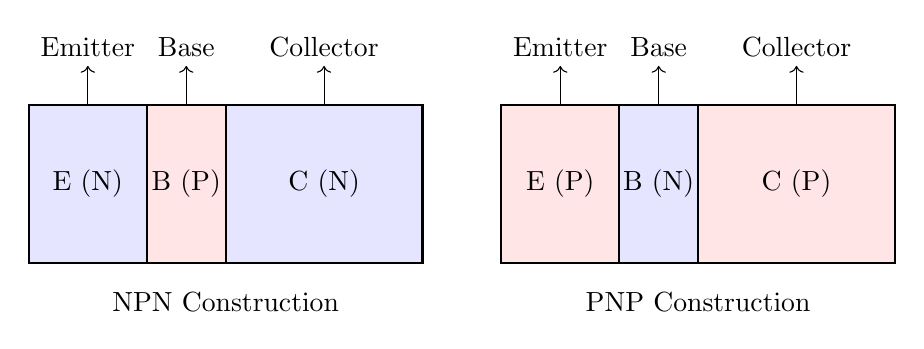
\begin{tikzpicture}
    % NPN
    \begin{scope}[xshift=0cm]
        \draw[thick, fill=blue!10] (0,0) rectangle (1.5, 2) node[midway] {E (N)};
        \draw[thick, fill=red!10] (1.5,0) rectangle (2.5, 2) node[midway] {B (P)};
        \draw[thick, fill=blue!10] (2.5,0) rectangle (5, 2) node[midway] {C (N)};
        \draw[->] (0.75, 2) -- (0.75, 2.5) node[above] {Emitter};
        \draw[->] (2, 2) -- (2, 2.5) node[above] {Base};
        \draw[->] (3.75, 2) -- (3.75, 2.5) node[above] {Collector};
        \node at (2.5, -0.5) {NPN Construction};
    \end{scope}

    % PNP
    \begin{scope}[xshift=6cm]
        \draw[thick, fill=red!10] (0,0) rectangle (1.5, 2) node[midway] {E (P)};
        \draw[thick, fill=blue!10] (1.5,0) rectangle (2.5, 2) node[midway] {B (N)};
        \draw[thick, fill=red!10] (2.5,0) rectangle (5, 2) node[midway] {C (P)};
        \draw[->] (0.75, 2) -- (0.75, 2.5) node[above] {Emitter};
        \draw[->] (2, 2) -- (2, 2.5) node[above] {Base};
        \draw[->] (3.75, 2) -- (3.75, 2.5) node[above] {Collector};
        \node at (2.5, -0.5) {PNP Construction};
    \end{scope}
\end{tikzpicture}
\end{answerdiagram}
\end{solutionbox}

\begin{mnemonicbox}
\mnemonic{ENB-CPM: Emitter has N in NPN, Collector is Proportionally Medium-doped}
\end{mnemonicbox}

% Question 5
\questionmarks{5(a)}{3}{Explain e-waste in brief.}

\begin{solutionbox}
\textbf{Answer}:

\textbf{E-Waste (Electronic Waste)}: Discarded electronic devices (phones, PCs, TVs).

\begin{itemize}
    \item \keyword{Hazards}: Contains toxic lead, mercury, cadmium.
    \item \keyword{Value}: Contains recoverable gold, silver, copper.
    \item \keyword{Impact}: Environmental pollution if ended in landfill.
    \item \keyword{Need}: Proper recycling and disposal management.
\end{itemize}
\end{solutionbox}

\begin{mnemonicbox}
\mnemonic{TECH: Toxic Electronics Create Hazards}
\end{mnemonicbox}

\questionmarks{5(b)}{4}{Illustrate operation of NPN transistor with figure.}

\begin{solutionbox}
\textbf{Answer}:

\textbf{Working Principle}:
\begin{itemize}
    \item \keyword{Forward Biased} Base-Emitter: Electrons injected from Emitter to Base.
    \item \keyword{Reverse Biased} Base-Collector: Electrons swept from Base to Collector.
    \item Small Base current ($I_B$) controls large Collector current ($I_C$).
    \item Equation: $I_E = I_B + I_C$.
\end{itemize}

\begin{answerdiagram}{NPN Operation}
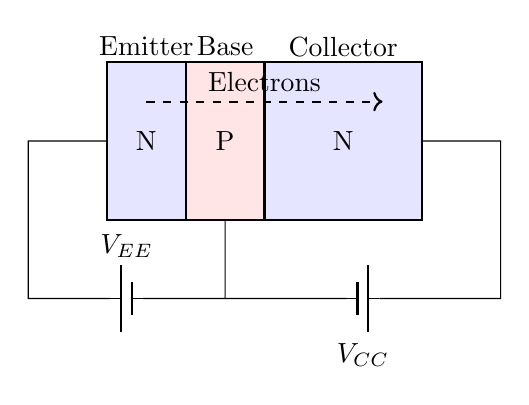
\begin{tikzpicture}
    % Block
    \draw[thick, fill=blue!10] (0,0) rectangle (1,2) node[midway] {N};
    \draw[thick, fill=red!10] (1,0) rectangle (2,2) node[midway] {P};
    \draw[thick, fill=blue!10] (2,0) rectangle (4,2) node[midway] {N};
    
    % Biasing batteries
    \draw (0,1) -- (-1,1) -- (-1, -1) to[battery1, l=$V_{EE}$] (1.5, -1) -- (1.5, 0);
    \draw (4,1) -- (5,1) -- (5, -1) to[battery1, l=$V_{CC}$] (1.5, -1);
    
    % Electron flow
    \draw[->, dashed, thick] (0.5, 1.5) -- (3.5, 1.5) node[midway, above] {Electrons};
    
    \node at (0.5, 2.2) {Emitter};
    \node at (1.5, 2.2) {Base};
    \node at (3, 2.2) {Collector};
\end{tikzpicture}
\end{answerdiagram}
\end{solutionbox}

\begin{mnemonicbox}
\mnemonic{BECAN: Base current Enables Collector Amplification in NPN}
\end{mnemonicbox}

\questionmarks{5(c)}{7}{Illustrate common emitter (CE) configuration of Transistor with input and output characteristics.}

\begin{solutionbox}
\textbf{Answer}:

\textbf{CE Configuration}: Emitter is grounded (common). Input at Base, Output at Collector. High Gain.

\begin{answerdiagram}{CE Circuit and Characteristics}
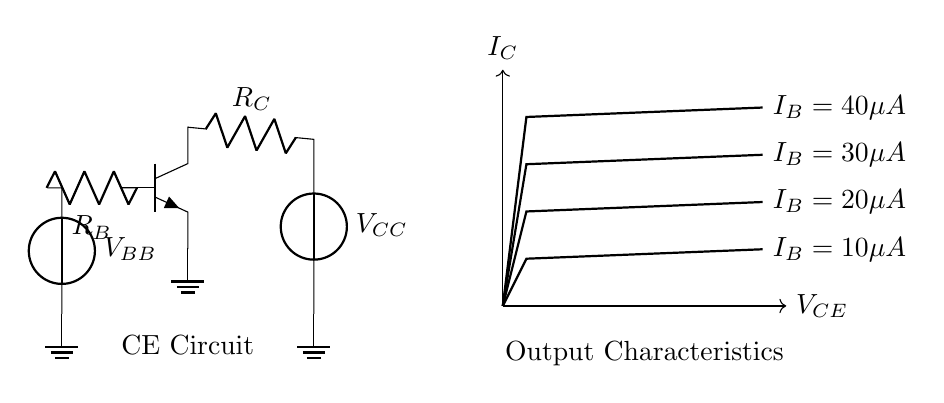
\begin{tikzpicture}
    % Circuit
    \begin{scope}[scale=0.8]
        \draw (0,0) node[npn](T){};
        \draw (T.E) node[ground]{};
        \draw (T.B) to[R, l=$R_B$] (-2,0) to[V, l=$V_{BB}$] (-2,-2) node[ground]{};
        \draw (T.C) to[R, l=$R_C$] (2,0.77) to[V, l=$V_{CC}$] (2,-2) node[ground]{};
        \node at (0, -2.5) {CE Circuit};
    \end{scope}

    % Output Characteristics
    \begin{scope}[xshift=4cm, yshift=-1.5cm, scale=0.6]
        \draw[->] (0,0) -- (6,0) node[right] {$V_{CE}$};
        \draw[->] (0,0) -- (0,5) node[above] {$I_C$};
        
        \draw[thick] (0,0) -- (0.5, 4) -- (5.5, 4.2) node[right] {$I_B=40\mu A$};
        \draw[thick] (0,0) -- (0.5, 3) -- (5.5, 3.2) node[right] {$I_B=30\mu A$};
        \draw[thick] (0,0) -- (0.5, 2) -- (5.5, 2.2) node[right] {$I_B=20\mu A$};
        \draw[thick] (0,0) -- (0.5, 1) -- (5.5, 1.2) node[right] {$I_B=10\mu A$};
        
        \node at (3, -1) {Output Characteristics};
    \end{scope}
\end{tikzpicture}
\end{answerdiagram}

\begin{itemize}
    \item \keyword{Input Char}: $I_B$ vs $V_{BE}$. Like a diode.
    \item \keyword{Output Char}: $I_C$ vs $V_{CE}$. Saturation (steep rise), Active (flat), Cutoff (zero).
\end{itemize}
\end{solutionbox}

\begin{mnemonicbox}
\mnemonic{CASIO: Common emitter Amplifies Signals with Inverted Output}
\end{mnemonicbox}

% Question 5 OR
\questionmarks{5(a) OR}{3}{State types of e-waste.}

\begin{solutionbox}
\textbf{Answer}:

\begin{itemize}
    \item \keyword{IT \& Telecom}: Computers, phones, printers.
    \item \keyword{Consumer}: TVs, audio sets, cameras.
    \item \keyword{Appliances}: Fridges, washing machines.
    \item \keyword{Lighting}: Bulbs, LEDs.
    \item \keyword{Medical}: Scanners, monitors.
\end{itemize}
\end{solutionbox}

\begin{mnemonicbox}
\mnemonic{CLIMATE: Computing, Lighting, Industrial, Medical, Appliances, Telecom, Electronic components}
\end{mnemonicbox}

\questionmarks{5(b) OR}{4}{Illustrate different categories of Electronics waste.}

\begin{solutionbox}
\textbf{Answer}:

\begin{center}
\captionof{table}{E-Waste Categories}
\begin{tabulary}{\linewidth}{|L|L|}
\hline
\textbf{Category} & \textbf{Examples} \\ \hline
Large Appliances & Washing machines, AC units \\ \hline
Small Appliances & Toasters, Irons \\ \hline
IT Equipment & PCs, Laptops, Mobile phones \\ \hline
Consumer Electronics & TVs, Stereos, Game consoles \\ \hline
Lighting & Fluorescent tubes \\ \hline
Tools & Drills, Saws \\ \hline
\end{tabulary}
\end{center}

\begin{answerdiagram}{E-Waste Composition}
\begin{tikzpicture}
    \pie[text=legend, radius=2, color={blue!20, red!20, green!20, orange!20, yellow!20}]{
        30/Large Appliances,
        25/IT \& Telecom,
        15/Consumer,
        15/Small Appliances,
        15/Others
    }
\end{tikzpicture}
\end{answerdiagram}
\end{solutionbox}

\begin{mnemonicbox}
\mnemonic{LIMCEST: Large, IT, Medical, Consumer, Electronic tools, Small, Telecom}
\end{mnemonicbox}

\questionmarks{5(c) OR}{7}{Explain transistor as a switch in cutoff and saturation region.}

\begin{solutionbox}
\textbf{Answer}:

\textbf{Transistor Switch States}:
\begin{center}
\begin{tabulary}{\linewidth}{|L|L|L|}
\hline
\textbf{State} & \textbf{Region} & \textbf{Conditions} \\ \hline
\textbf{OFF (Open)} & \keyword{Cutoff} & $V_{in} < 0.7V$, $I_B=0$, $I_C=0$, $V_{CE}=V_{CC}$. \\ \hline
\textbf{ON (Closed)} & \keyword{Saturation} & $V_{in} > 0.7V$, $I_B$ max, $I_C$ max, $V_{CE} \approx 0.2V$. \\ \hline
\end{tabulary}
\end{center}

\begin{answerdiagram}{Transistor Switching}
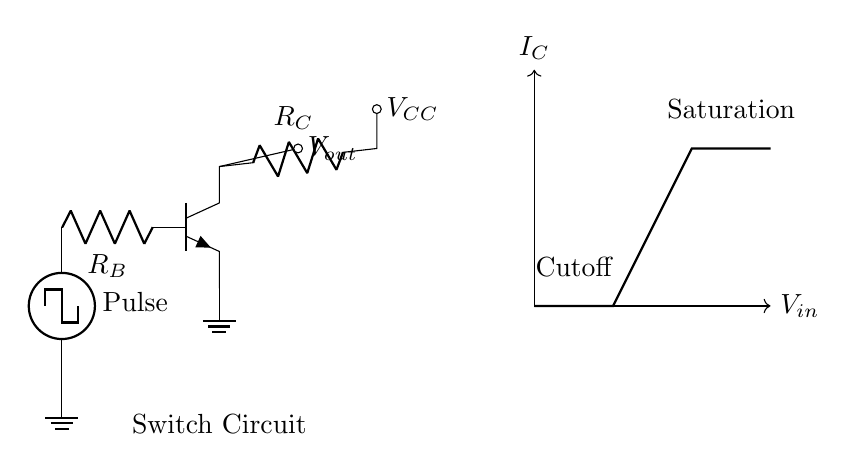
\begin{tikzpicture}
    % Circuit
    \begin{scope}
        \draw (0,0) node[npn](T){};
        \draw (T.E) node[ground]{};
        \draw (T.B) to[R, l=$R_B$] (-2,0) to[sqV, l=Pulse] (-2,-2) node[ground]{};
        \draw (T.C) to[R, l=$R_C$] (2,1) to[short, -o] (2,1.5) node[right]{$V_{CC}$};
        \draw (T.C) to[short, -o] (1,1) node[right]{$V_{out}$};
        
        \node at (0, -2.5) {Switch Circuit};
    \end{scope}

    % Graph
    \begin{scope}[xshift=4cm, yshift=-1cm]
        \draw[->] (0,0) -- (3,0) node[right]{$V_{in}$};
        \draw[->] (0,0) -- (0,3) node[above]{$I_C$};
        \draw[thick] (0,0) -- (1,0) -- (2,2) -- (3,2);
        \node at (0.5, 0.5) {Cutoff};
        \node at (2.5, 2.5) {Saturation};
    \end{scope}
\end{tikzpicture}
\end{answerdiagram}
\end{solutionbox}

\begin{mnemonicbox}
\mnemonic{COSVL: Cutoff means Off State with Vce Large}
\end{mnemonicbox}

\end{document}

